\chapter{Análise de resultados}
 O objetivo do projeto é o desenvolvimento de uma aplicação \textit{mobile} com foco na área do fórum, pelo que, este deve permitir o registo de empresas, gestão de utilizadores, notificações, comunicações por \textit{email}, gestão de conta e notificações do utilizador.



 \section{Tarefas}

A nível de tarefas, o esperado, como mencionado no capítulo \ref{sec:planificacao trabalho}, seria terminar o projeto no final de março, o que não se tornou realidade, visto que, diversos imprevistos ocorreram no caminho, sendo o principal o atraso no desenvolvimento do \textit{webscraper}. Este atraso derivou da constante atualização do catálogo, o que levava a alterações no conteúdo do \textit{website}, sendo necessário alterar o código de leitura a cada alteração. Outro grande problema encontrado foi a alteração de alguns requisitos durante o desenvolvimento, o que resultou em mais tarefas e por si, mais tempo de desenvolvimento.

Estes imprevistos e dificuldades no desenvolvimento levaram a um atraso de um mês e uma semana, estava previsto concluir o projeto em março, mas, contudo, apenas foi finalizado no início de maio.

Apesar de todas as dificuldades, todas as tarefas previstas foram concluídas.

\begin{figure}[htb]
 \centering
 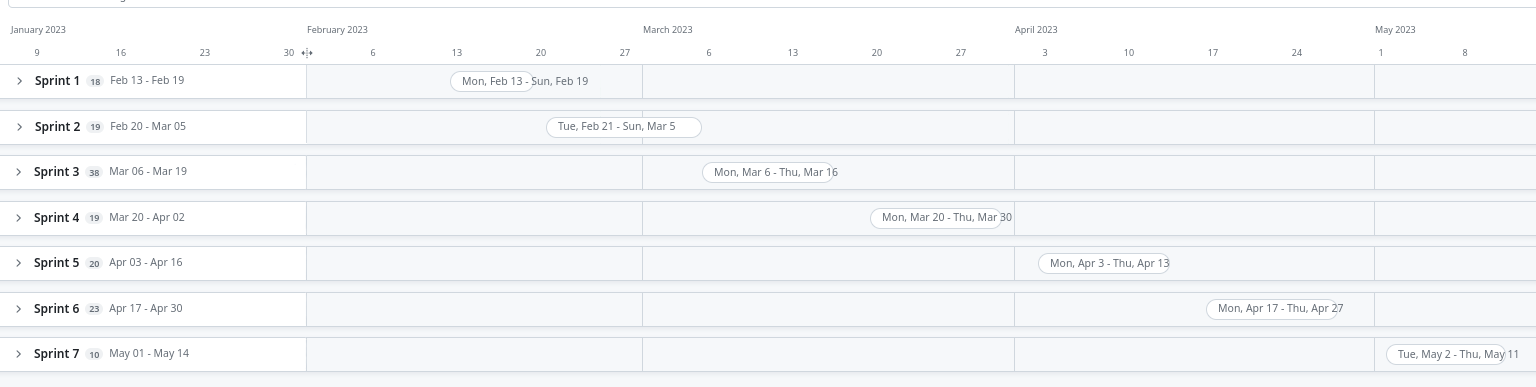
\includegraphics[width=\textwidth]{images/analise_resultados/planeamento_final.png}
 \caption{Organização de tarefas final}
 \label{fig:78}
\end{figure}

\newpage

\section{Base de dados}

Um dos pontos que sofreu mais alterações durante o desenvolvimento do projeto foi a base de dados, pois, com alteração dos requisitos e do catálogo dos produtos foi necessário realizar várias alterações até alcançar a versão final.

\begin{figure}[htb]
 \centering
 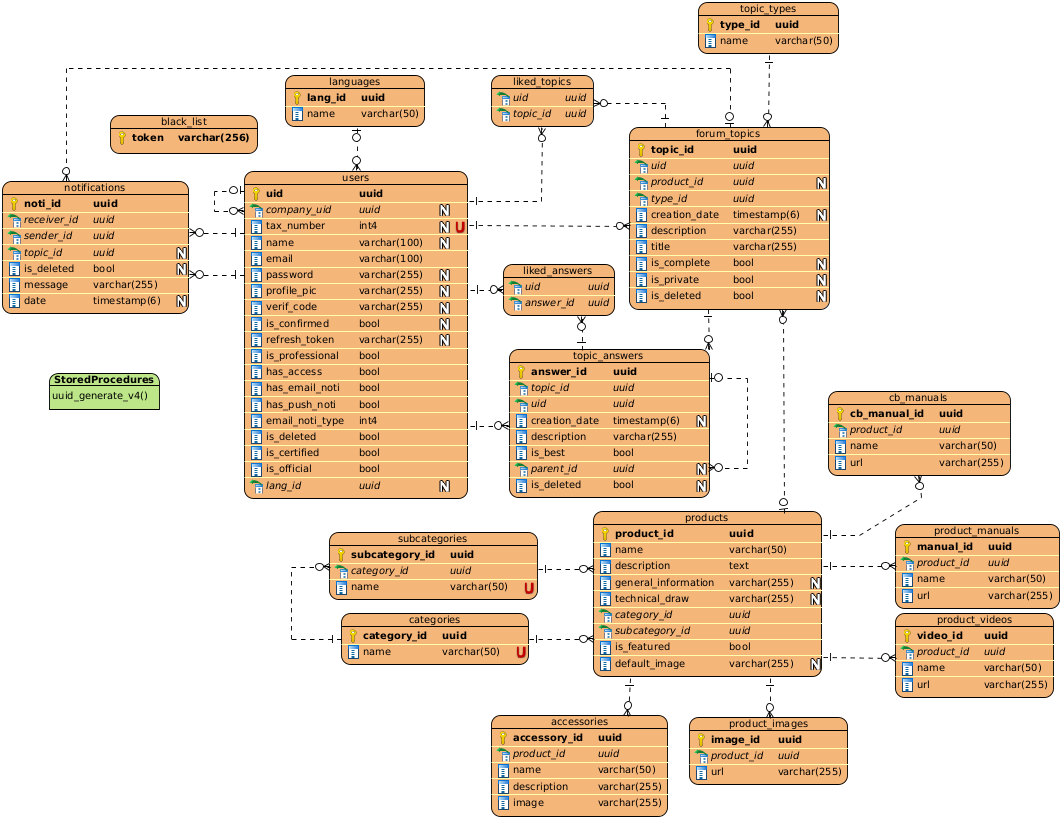
\includegraphics[width=0.7\textwidth]{images/diagramas/diagrama_bd.png}
 \caption{Base de dados inicial}
 \label{fig:79}
\end{figure}

\begin{figure}[htb]
 \centering
 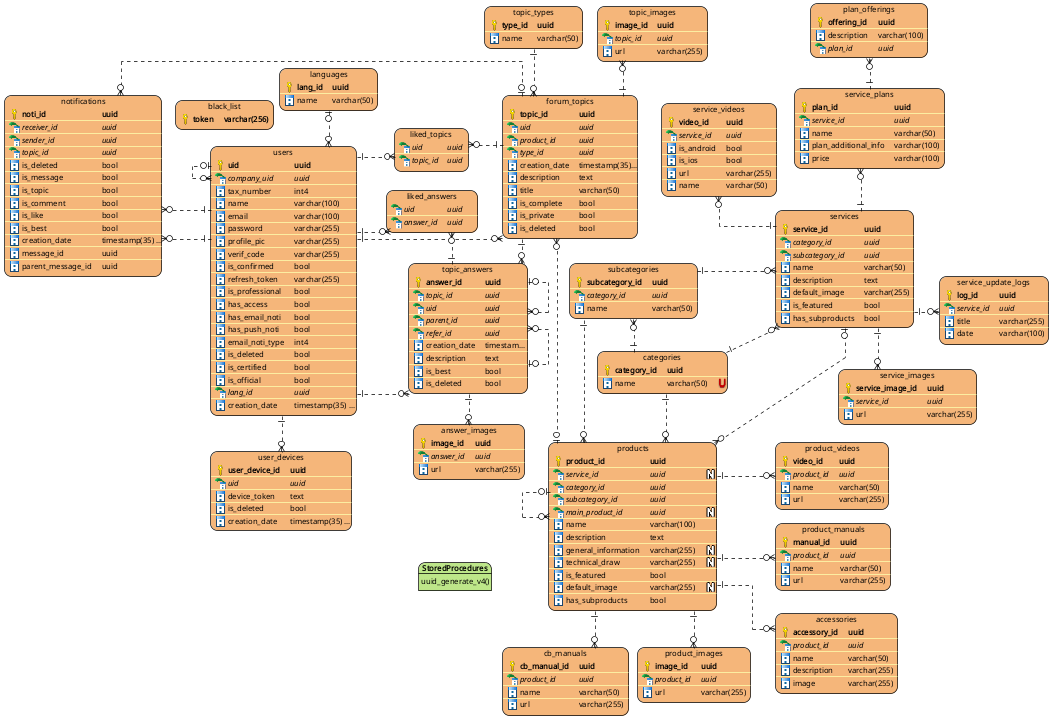
\includegraphics[width=0.7\textwidth]{images/diagramas/bd_final.png}
 \caption{Base de dados final}
 \label{fig:80}
\end{figure}


\section{Aplicação final}
Já na aplicação final, todos os parâmetros estipulados foram alcançados, sendo apenas alguns pontos alterados, como por exemplo, as categorias de tópicos, que foram alteradas de forma a que as categorias mais importantes fossem apresentadas.


\section{Opinião do cliente}

Após o desenvolvimento do projeto foi apresentado ao cliente o resultado final para este realizar uma verificação se tudo encontrava-se conforme os requisitos e expectativas.

 Na apresentação, o cliente dispôs de uma opinião positiva, com a indicação de que a aplicação encontrava-se conforme as expectativas e requisitos. O único ponto em falta é a testagem da solução em relação a erros e desempenho, sendo que, só poderá ser realizada após a aplicação ser lançada, dado que, não foi possível realizar testes em larga escala.